\section{Results}
In this short section we will revisit the model of \cite{huberman_evolutionary_1993} mentioned in the introduction and present results simulating it with our four update-strategies. 

\subsection{Prisoners Dilemma}
\begin{figure*}
        \centering
        \begin{subfigure}[b]{0.475\textwidth}
            \centering
            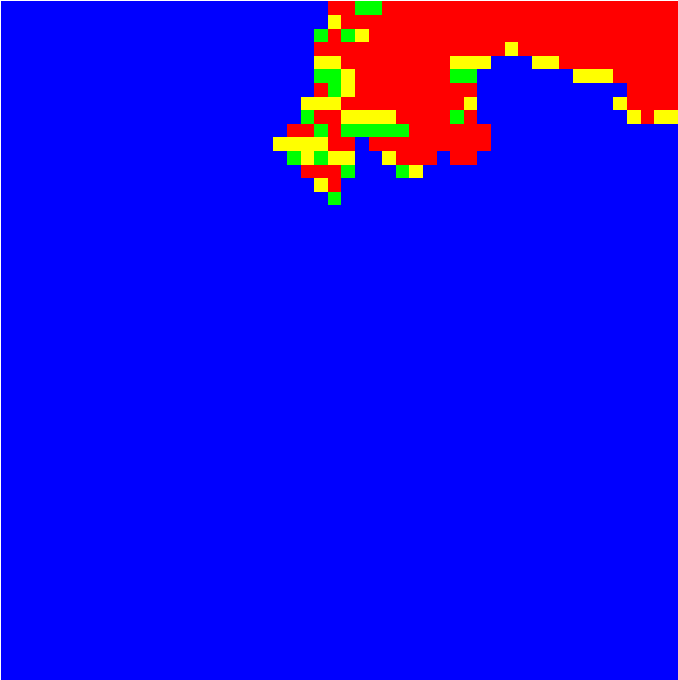
\includegraphics[width=.4\textwidth, angle=0]{./fig/seq_50x50_45steps_MSG_haskell.png}
            \caption[]%
            {{\small Sequential Strategy}}    
            \label{fig:seq_strat}
        \end{subfigure}
        \hfill
        \begin{subfigure}[b]{0.475\textwidth}  
            \centering 
            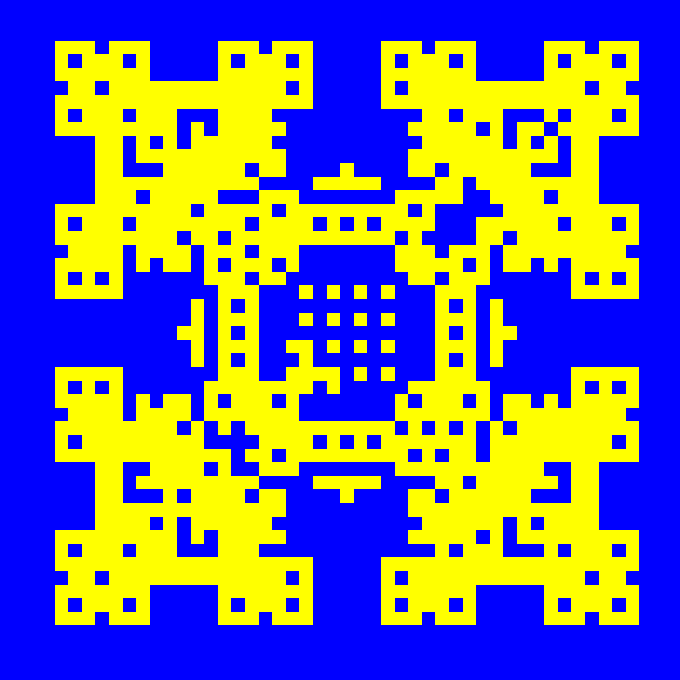
\includegraphics[width=.4\textwidth, angle=0]{./fig/par_50x50_45steps_MSG_haskell.png}
            \caption[]%
            {{\small Parallel Strategy}}    
            \label{fig:par_strat}
        \end{subfigure}
        \vskip\baselineskip
        \begin{subfigure}[b]{0.475\textwidth}   
            \centering 
            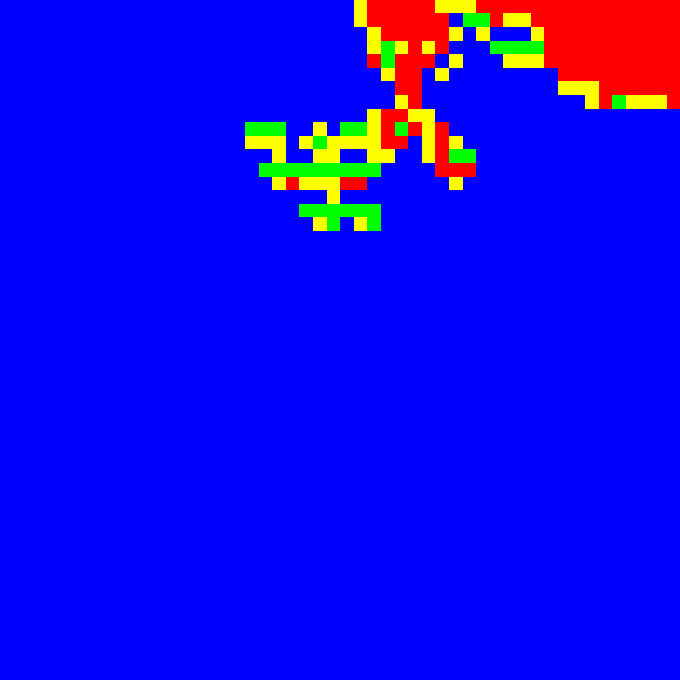
\includegraphics[width=.4\textwidth, angle=0]{./fig/con_50x50_45steps_MSG_haskell.png}
            \caption[]%
            {{\small Concurrent Strategy}}    
            \label{fig:con_strat}
        \end{subfigure}
        \quad
        \begin{subfigure}[b]{0.475\textwidth}   
            \centering 
            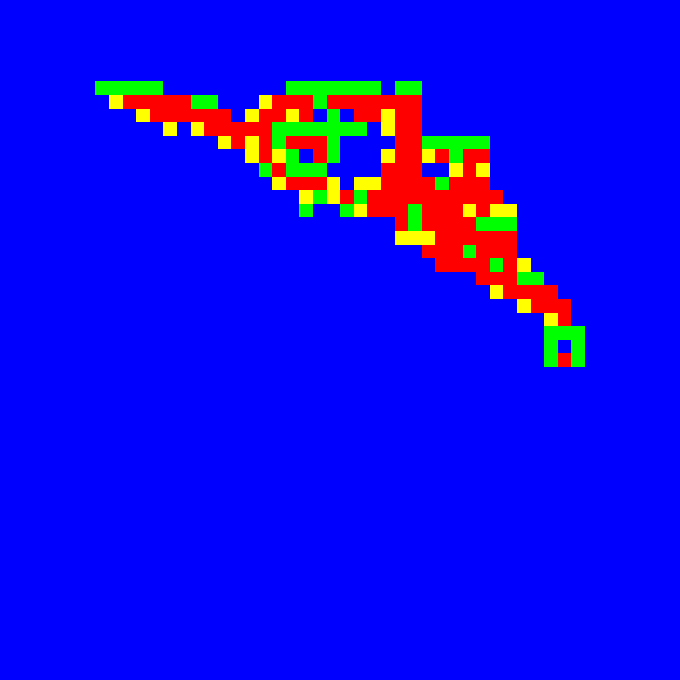
\includegraphics[width=.4\textwidth, angle=0]{./fig/act_50x50_45steps_MSG_haskell.png}
            \caption[]%
            {{\small Actor Strategy}}    
            \label{fig:act_strat}
        \end{subfigure}
        \caption[]
        {\small Haskell implementation of Prisoner-Dilemma game as in \cite{huberman_evolutionary_1993} on a 50x50 grid after 45 steps.} 
        \label{fig:prisoner_strategies}
    \end{figure*}
    
It is immediate clear that, when looking at figure \ref{fig:prisoner_strategies} the update-strategy which reflects the semantics of the model is the Parallel Strategy as all others clearly fail to reproduce the pattern as predicted by the model. Thus we can say only the Parallel Strategy is suitable to simulate this model and that only this Strategy is the correct one. \\
The reason why the others fail to reproduce the pattern is due to the non-parallel and unsynchronized way that information spreads through the grid: in the Sequential Strategy the Agents further ahead in the queue play the game earlier and influence the neighbourhood thus Agents in the neighbourhood which play the game later find an already changed environment/messages and act thus based upon these informations. This is not the case in the Parallel version: all Agents play the game on the frozen state of the previous step and the outcome of each Agents game will only be visible in the next step. In the Concurrent and Actor Strategy the Agents run in parallel but changes are visible immediately and concurrently, thus leading to the same non-structural patterns as in the Sequential Strategy. \\
Note that the Concurrent and Actor Strategy produce different results on every run due to the inherent non-deterministic event-ordering introduce by concurrency. Also note that it is not possible to calculate 45 steps for the Actor Strategy as it lacks the Global Synchronization property. To arrive at a relative comparative result we just waited until the first Agent arrives at a local time of 45 and then rendered the result. 

\subsection{Heroes \& Cowards}
To study various properties of implementations of ABS we select the very simple model \textit{Heroes \& Cowards} from social-simulation invented by \cite{wilensky_introduction_2015}. Although it is very simple, it will prevent the research of the methods to be cluttered with too many subtle details of the model thus focusing on the methods and implementation than rather on the model itself. \\
One starts with a crowd of Agents where each Agent is positioned \textit{randomly} in a continuous 2D-space. Each of the Agents then selects \textit{randomly} one friend and one enemy (except itself in both cases) and decides with a given probability whether the Agent acts in the role of a "Hero" or a "Coward" - friend, enemy and role don't change after the initial set-up. Now the simulation can start: in each step the Agent will move a given distance towards a given point. If the Agent is in the role of a "Hero" this point will be the half-way distance between the Agents friend and enemy - the Agent tries to protect the friend from the enemy. If the Agent is acting like a "Coward" it will try to hide behind the friend also the half-way distance between the Agents friend and enemy, just in the opposite direction. \\
The world this model is situated in is restricted by borders in the form of a rectangle: the agents cannot move out of it and will be clipped against the border if the calculation would end them up outside. \\
Note that this simulation is determined by the random starting positions, random friend \& enemy selection, random role selection and number of agents. Note also that during the simulation-stepping no randomness is mentioned in the model and given the initial random set-up, the simulation-\textit{model} is completely deterministic - whether this is the case for the implementations is another question, not relevant to the model. 

TODO: show results with heroes \& cowards in java with 100.000 agents after 500 (?) steps